\documentclass[tikz,border=15pt]{standalone}
\usepackage{tikz}
\usepackage{xcolor}
\usetikzlibrary{arrows.meta,calc}

\definecolor{bgcolor}{RGB}{15,23,42}
\definecolor{cardbg}{RGB}{30,41,59}
\definecolor{cardborder}{RGB}{51,65,85}
\definecolor{cyanlight}{RGB}{56,189,248}
\definecolor{cyandark}{RGB}{2,132,199}
\definecolor{slateaxis}{RGB}{148,163,184}
\definecolor{slatedim}{RGB}{100,116,139}
\definecolor{rosevector}{RGB}{244,63,94}
\definecolor{goldphi}{RGB}{251,191,36}
\definecolor{indigolabel}{RGB}{165,180,252}

\begin{document}
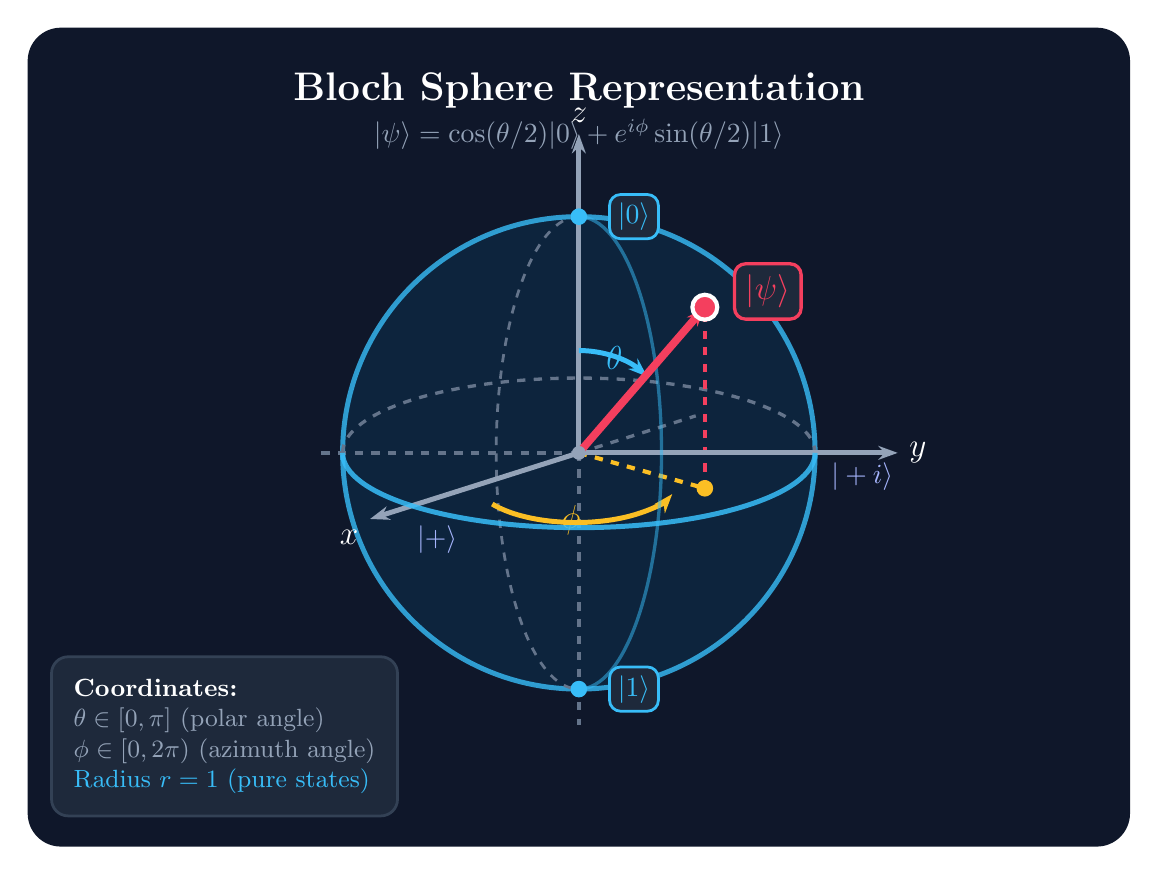
\begin{tikzpicture}[
    >={Stealth[length=7pt, width=5pt]}
]

% Background Card
\fill[rounded corners=12pt, fill=bgcolor] (-7.0,-5.2) rectangle (7.0,5.2);

% Title & Formula
\node[text=white, font=\Large\bfseries] at (0, 4.4) {Bloch Sphere Representation};
\node[text=slateaxis, font=\normalsize\itshape] at (0, 3.85) {$|\psi\rangle = \cos(\theta/2)|0\rangle + e^{i\phi}\sin(\theta/2)|1\rangle$};

% Radius & Centers
\def\R{3.0}
\def\ry{0.95}
\def\rx{1.05}

% Center at (0, -0.2)
\coordinate (O) at (0, -0.2);

% Sphere Shading & Outer Circle
\fill[fill=cyandark, opacity=0.12] (O) circle (\R);
\draw[draw=cyanlight, line width=1.8pt, opacity=0.8] (O) circle (\R);

% Back Equator & Meridian (Dashed)
\draw[slatedim, line width=1.2pt, dashed] ($(O)+(-\R, 0)$) arc (180:0:{\R} and {\ry});
\draw[slatedim, line width=1.0pt, dashed] ($(O)+(0, \R)$) arc (90:270:{\rx} and {\R});

% Negative Axes (Dashed)
\draw[slatedim, line width=1.2pt, dashed] (O) -- ($(O)+(0, -\R*1.15)$);
\draw[slatedim, line width=1.2pt, dashed] (O) -- ($(O)+(-\R*1.1, 0)$);
\draw[slatedim, line width=1.2pt, dashed] (O) -- ($(O)+({0.7*\R*cos(45)}, {0.7*\ry*sin(45)})$);

% Equatorial Projection of |psi>
\coordinate (PSI_PROJ) at ($(O)+(1.6, -0.45)$);
\coordinate (PSI) at ($(O)+(1.6, 1.85)$);

\draw[goldphi, line width=1.5pt, dashed] (O) -- (PSI_PROJ);
\draw[rosevector, line width=1.5pt, dashed] (PSI_PROJ) -- (PSI);
\fill[goldphi] (PSI_PROJ) circle (3pt);

% Angle phi arc on xy-plane
\draw[goldphi, line width=1.8pt, ->] ($(O)+(-1.1, -0.65)$) arc (-145:-20:1.3 and 0.55);
\node[text=goldphi, font=\large\bfseries\itshape] at ($(O)+(-0.1, -0.85)$) {$\phi$};

% Positive Axes
% +x Axis (forward-left)
\draw[slateaxis, line width=1.8pt, ->] (O) -- ($(O)+({-1.25*\R*cos(45)}, {-1.25*\ry*sin(45)})$) node[below left, text=white, font=\large\bfseries] {$x$};
% +y Axis (right)
\draw[slateaxis, line width=1.8pt, ->] (O) -- ($(O)+(\R*1.35, 0)$) node[right, text=white, font=\large\bfseries] {$y$};
% +z Axis (up)
\draw[slateaxis, line width=1.8pt, ->] (O) -- ($(O)+(0, \R*1.35)$) node[above, text=white, font=\large\bfseries] {$z$};

% Front Equator & Meridian (Solid)
\draw[cyanlight, line width=1.8pt, opacity=0.85] ($(O)+(-\R, 0)$) arc (180:360:{\R} and {\ry});
\draw[cyanlight, line width=1.2pt, opacity=0.5] ($(O)+(0, \R)$) arc (90:-90:{\rx} and {\R});

% Angle theta arc
\draw[cyanlight, line width=1.8pt, ->] ($(O)+(0, 1.3)$) arc (90:48:1.3);
\node[text=cyanlight, font=\large\bfseries\itshape] at ($(O)+(0.45, 1.2)$) {$\theta$};

% State Vector |psi>
\draw[rosevector, line width=2.8pt, ->] (O) -- (PSI);
\fill[fill=rosevector, draw=white, line width=1.5pt] (PSI) circle (4.5pt);

% |psi> Label Box
\node[fill=cardbg, draw=rosevector, line width=1.2pt, rounded corners=4pt, text=rosevector, font=\large\bfseries, inner sep=4pt] at ($(PSI)+(0.8, 0.2)$) {$|\psi\rangle$};

% North Pole |0>
\fill[cyanlight] ($(O)+(0, \R)$) circle (3pt);
\node[fill=cardbg, draw=cyanlight, line width=1pt, rounded corners=4pt, text=cyanlight, font=\normalsize\bfseries, inner sep=3pt] at ($(O)+(0.7, \R)$) {$|0\rangle$};

% South Pole |1>
\fill[cyanlight] ($(O)+(0, -\R)$) circle (3pt);
\node[fill=cardbg, draw=cyanlight, line width=1pt, rounded corners=4pt, text=cyanlight, font=\normalsize\bfseries, inner sep=3pt] at ($(O)+(0.7, -\R)$) {$|1\rangle$};

% Other Basis States
\node[text=indigolabel, font=\normalsize\bfseries] at ($(O)+(-1.8, -1.1)$) {$|+\rangle$};
\node[text=indigolabel, font=\normalsize\bfseries] at ($(O)+(\R+0.6, -0.3)$) {$|+i\rangle$};

% Origin
\fill[slateaxis] (O) circle (2.5pt);

% Info Box (Bottom Left)
\node[fill=cardbg, draw=cardborder, line width=1pt, rounded corners=6pt, text=slateaxis, font=\small, align=left, inner sep=8pt] at (-4.5, -3.8) {
    \textbf{\textcolor{white}{Coordinates:}}\\
    $\theta \in [0, \pi]$ (polar angle)\\
    $\phi \in [0, 2\pi)$ (azimuth angle)\\
    \textcolor{cyanlight}{Radius $r=1$ (pure states)}
};

\end{tikzpicture}
\end{document}
